\chapter{Breaching Active Directory}

\begin{abstract}
Active Directory (AD) underpins identity and access management for the majority of enterprise Windows environments, with approximately 90\% of Global Fortune 1000 companies relying on it. As the dominant suite for managing Windows domain-based networks, AD orchestrates authentication, authorization, and policy enforcement across an organization's entire IT estate. This central role makes AD both indispenable and a prime target for adversaries-compromise of AD effectively grants an attacker "keys to the kingdom," enabling lateral movement, privilege escalation, and persistent access.

Two of the most common attack vectors for obtaining initial AD credentials are Open-Source Intelligence (OSINT) and phishing. OSINT leverages publicly available information-from corporate websites, social media, data breaches, and other online sources-to identify likely usernames, email formats, or even leaked password hashes and fragments. Phishing, by contrast, uses deceptive communications, often via email or SMS, to trick users into revealing credentials or executing malicious payloads. Both methods bypass traditional perimeter defenses and exploit human factors, underscoring the need for defender's to better safeguard their AD territories by proactively implemented layered defense in depth security measures.
\end{abstract}
This chapter examines the prevalence of AD in enterprise emvironments, the high-value nature of its compromise, and the operational realities of OSINT and phishing as entry points. By analyzing attacker methodologies and defensive flaws, gaps, and weaknesses, it highlights the necessity for layered security controls, user awareness training, and continuous monitoring to protect the integrity of enterprise identity infrastructure that is Active Directory (AD).

\section{NTLM Authentication Services}
\textit{New Technology LAN Manager (NTLM)} is a suite of Microsoft security protocols that facilitate authentication, integrity, and confidentiality for users within an Active Directory (AD) environment. It remains a legacy authentication mechanism, yet it is still widely present in modern enterprise networks due to backward compatibility requirements and the sheer number of services that rely on it.

A core component of NTLM-based authentication is \textit{NetNTLM,} which implements a challenge-response authentication model. This mechanism is frequently used by both internal and external public internet-facing network services. Within an internal network, NetNTLM plays a crucial role in allowing applications and services to authenticate users without directly handling sensitive password data; however, a critical security consideration is that some services using NetNTLM are exposed to the internet-deliberately or inadvertently-making them potential entry points for attackers.

Common examples of internet-exposed services that use NetNTLM include:
\begin{itemize}
    \item \textbf{Internally-hosted Microsoft Exchange email servers} that present an Outlook Web Application (OWA) login portal to users over the Internet.
    \item \textbf{Remote Desktop Protocol (RDP) services} that are made publicly accessible, often for remote administration or user access.
    \item \textbf{Virtual Private Network (VPN) endpoints} integrated with AD for user authentication.
    \item \textbf{Internet-facing web applications} that rely on Windows Authentication (NetNTLM) for login functionality.
\end{itemize}

NetNTLM-sometimes simply referred to as \textit{"Windows Authentication"} or \textit{"NTLM Authentication"}- operates by positioning the application as an intermediary between the client and the Domain Controller (DC). When a user attempts to authenticate, the application does not verify the credentials itself. Instead, it forwards authentication data to the DC in the form of a cryptographic challenge. If the DC verifies the response as correct, the application grants the user access.

This design ensures that the application never stores or processes plaintext AD credentials directly, reducing the risk of credential theft from the application's own storage or logs. In theory, only the Domain Controller ever has the capability to validate the actual credentials, preserving the security of the authentication process.

This intermediary model is an important security safeguard, but it also introduces unique attack vectors-particularly if the services are exposed to the internet. Attackers can exploit such exposure to capture authentication exchanges or relay them to other services, potentially leading to unauthorized access.

This process is illustrated in the diagram below:
\begin{figure}
    \centering
    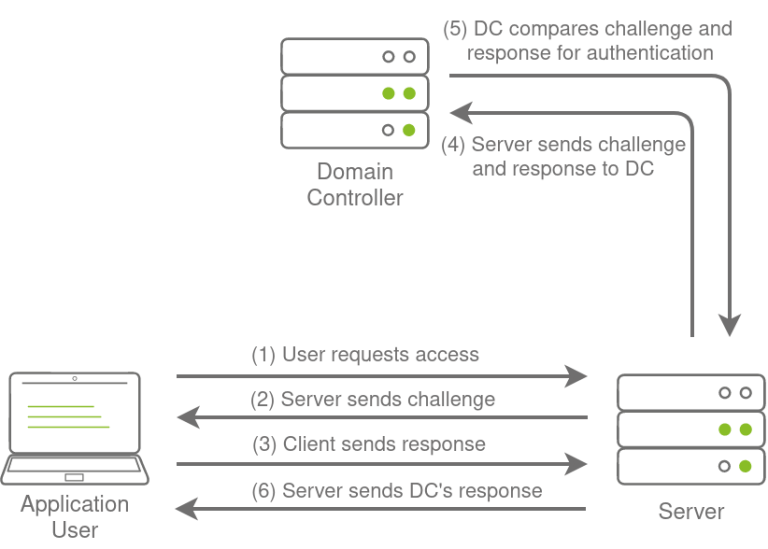
\includegraphics[width=0.75\linewidth]{1ntlmauth.png}
    \caption{NTLM authentication request process}
    \label{fig:placeholder}
\end{figure}
\section{Brute-Force Login Attacks}
In an Active Directory (AD) environment, traditional brute-force attacks-where an attacker systematically attempts many password combinations for a single user account-are rarely effective in practice nowadays. This is because most organizations configure \textit{account lockout policies} that temporarily disable an account after a set number of consecutive failed login attempts. Such policies, while effective at stopping unlimited guessing on a single account, do not effectively eliminate the immediate threat of credential guessing entirely.

To bypass these lockout restrictions, attackers often turn to a more measured technique known as \textit{password spraying.} Unlike traditional brute-forcing, which targets one account with many passwords, password spraying attacks flips this approach: the attacker chooses a single password (or a very small subset of passwords) and attempts to authenticate against a large number of usernames contained within the domain. The list of usernames is retrieved by way of enumerating all users within the domain.

The effectiveness of this method lies in human behaviors. Users-across industries and organizations-often rely on weak, predictable, or reused passwords. Examples include seasonal variations (e.g., \textit{Summer2025!),} company names plus year, or common patterns like \textit{Welcome123.} Since the attacker is only testing one password per account in each pass, the account lockout mechanism is far less likely to be triggered. Over time, the attacker can rotate through a small list of candidate passwords, spacing out attempts to avoid detection and circumvent these lockout thresholds.

However, this tactic is not without risk to the attacker. Even when executed slowly and carefully, password spraying can produce a large volume of failed authentication attempts across many accounts. In a well-monitored environment, security teams can detect these anomalies through \textit{Security Information and Event Management (SIEM)} systems, Domain Controller event logs, or intrusion detection alerts. Common indicators include multiple failed logon attempts from a single source IP, a pattern of failed attempts spread evenly across many accounts, or repeated attempts against inactive or disabled accounts.

When password spraying is successful, the attacker obtains valid AD credentials without triggering a lockout event. These credentials can then be used to access internal resources, move laterally, or escalate privileges. Because of this, password spraying remains a highly attractive option for attackers targeting AD-particularly when combined with prior username harvesting via OSINT, phishing, or enumeration of public services or the domain itself.

In sum, while brute-forcing login attempts in the traditional sense are mostly mitigated by lockout policies, password spraying sidesteps this defense and remains a common, real-world threat to enterprise authentication systems. Defenders must therefore focus not only on lockout configurations but also on proactive monitoring, user education, and enforcing strong, unique passwords across the estate.

\section{Password Spraying}
Password spraying is a targeted credential-guessing technique used against Active Directory environments to identify accounts with weak or commonly used passwords-without triggering account lockout mechanisms. Unlike traditional brute-force attacks, which attempt multiple passwords for a single user account, password spraying tests a single password (or a very small list) against a large number of domain-joined accounts.

The primary advantage for an attacker is \textit{stealth.} By limiting the number of attempts per account in each pass, they can greatly avoid triggering account lockout thresholds and alerts while still covering a large portion of the user populace. This is particularly effective when the attacker has already harvested usernames and gathered information through means of OSINT techniques, phishing, spearphishing campaigns, or enumeration techniques.

When targeting services that support NTLM authentication, attackers often use automated scripting tools to perform password spraying at scale. The example below demonstrates the use of a Python-based NTLM password spraying script:
\begin{lstlisting}
// Hello.java
import javax.swing.JApplet;
import java.awt.Graphics;

public class Hello extends JApplet {
    public void paintComponent(Graphics g) {
        g.drawString("Hello, world!", 65, 95);
    }    
}
\end{lstlisting}



















